\section{Results}
\label{sec:results}

Code and data are available at the Github repostitories here: \url{https://github.com/devangel77b/marcello-2020-code} and here: \url{https://github.com/devangel77b/marcello-manuscripts}. 

\subsection{Initial simulations of bio-inspired dive pullout maneuvers in \Matlab}
%if possible, add a sub-sub section for results
Using the modeling framework of \cite{hartman2014quadcopter}, four trials were run at varying speed reductions: a trial run at the actual hummingbird trajectory's speed, a trial at one fifth the hummingbird trajectory's speed, a trial at one tenth speed, and a trial at one twentieth speed relative to the full scale, full speed trajectories in \cite{clark2009courtship}. The results of those tests are shown in Figs.~\ref{fig:actualspeed}-\ref{fig:onetwentiethspeed}. Distance error calculations for the four trials are shown in \fref{tab:RMSE}. 
%reference the 4 trajectory path figures from actual speed to one twentieth
%why is this so not in the right place
%It also should be LARGER if at all possible. It's kind of tiny which makes it difficult to read
%Larger is tough - this is actually right size it should be same size font as text..normalyl would fit inside a column. 
\begin{table}[hb]
\caption{Distance error calculations for each trial (actual speed, one fifth speed, one tenth speed, and one twentieth speed). RMS position error, combining $x$ and $z$, is represented by the variable $e_p$, defined in \fref{eq:demonstration-1}.}
\label{tab:RMSE}
\begin{center}
%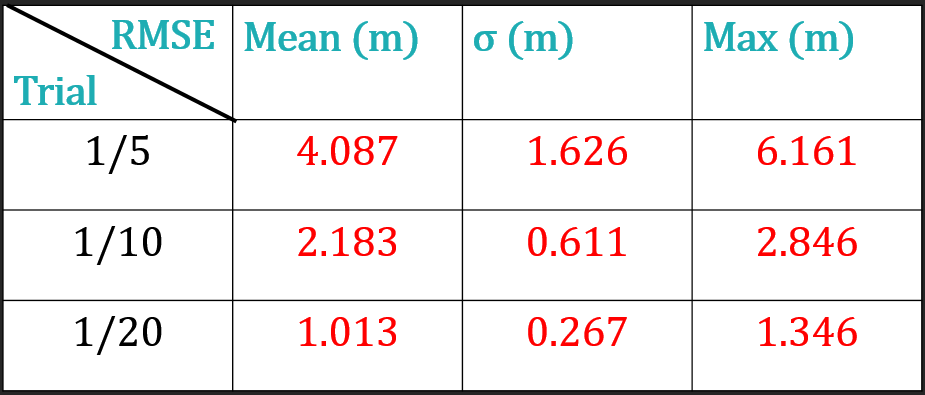
\includegraphics[width=0.6\columnwidth]{\myroot/figures/RMSEtable.png}
\begin{tabular}{cccc}
\toprule
Trial & $\overline{e_p}, \si{\meter}$ & $\sigma_{e_p}, \si{\meter}$ & $\max(e_p), \si{\meter}$  \\ %want absolute value bars or cap X to indicate a multi-dimension magnitude error and not only in the x direction --seems clear without, uglier with bars and e_p is defined before
\midrule
1 & 6.6888 & 4.3926 & 13.5984 \\
1/5 & 3.9415 & 1.8710 & 6.3231 \\
1/10 & 2.1757 & 0.7700 & 2.9967 \\
1/20 & 1.0443 & 0.3328 & 1.3603 \\
\bottomrule
\end{tabular}
\end{center}
\end{table}

For these experiments, the attitude angle command saturation limits were increased to $\pm\ang{45}$ to allow for larger command inputs to take advantage of a wider range of pitch angles. The simulated quadrotor was able to follow the one twentieth speed reduction the closest, and had the smallest RMSE, while the trial at one fifth the speed was incredibly behind the desired trajectory path. The trial at normal speed showed how inferior this control method is at executing high-speed extreme maneuvers, as the quadrotor was barely able to begin accelerating by the time the simulation called for the quadrotor to be completing the trajectory. As such, further experimentation with this controller at actual speed was discontinued, as it seems more relevant to focus on improving the control at slower speeds first before attempting improvment at full speed.

\clearpage
%These figures aren't showing up in subsection A like I want them to.....
%Figures here!!!! (4) with captions
% [p] makes it want to put it on a page of floats, so either clear a page to put them on
% or make them a little smaller
\begin{figure}[p]
\begin{center}
\includegraphics[width=0.6\columnwidth]{\myroot/figures/traj_1x.png}
\end{center}
\caption{Crazyflie attempted trajectory flight of the hummingbird trajectory at its actual speed.}
\label{fig:actualspeed}
\end{figure}

\begin{figure}[p]
\begin{center}
\includegraphics[width=0.6\columnwidth]{\myroot/figures/traj_5x.png}
\end{center}
\caption{Crazyflie attempted trajectory flight of the hummingbird trajectory at one fifth its actual speed.}
\label{fig:onefifthspeed}
\end{figure}

\clearpage
\begin{figure}[p]
\begin{center}
\includegraphics[width=0.6\columnwidth]{\myroot/figures/traj_10x.png}
\end{center}
\caption{Crazyflie attempted trajectory flight of the hummingbird trajectory at one tenth its actual speed.}
\label{fig:onetenthspeed}
\end{figure}

\begin{figure}[p]
\begin{center}
\includegraphics[width=0.6\columnwidth]{\myroot/figures/traj_20x.png}
\end{center}
\caption{Crazyflie attempted trajectory flight of the hummingbird trajectory at one twentieth its actual speed.}
\label{fig:onetwentiethspeed}
\end{figure}








% THE FOLLOWING IS NEW WORK DONE  ON GAIN TUNING AND RESULTING ERROR IMPROVEMENTS
\clearpage
\subsection{Improved control simulations of bio-inspired dive pullout maneuvers in \Matlab}
As discussed in the \fref{sec:methods}, several different attempts were made at improving the control of the quadrotor. The only method that proved successful enough to show meaningful visual results was the manual gain tuning. The results of which, for trials at one fifth speed, one tenth speed, and one twentieth speed, are compiled into the three figures shown below in \fref{fig:iconefifthspeed},~\fref{fig:iconetenthspeed}, and~\fref{fig:iconetwentiethspeed}. The new error calculations for these trials are also displayed in \fref{tab:icRMSE}. Additionally, the results of marginal analysis at each speed trial are displayed in \fref{tab:marginalanalysis}. Of note, the marginal analysis indicated that, for the trial at one twentieth the speed of the hummingbird trajectory, any changes made to the gain values (of five percent) only increased the overall root mean square error. This is represented in the table by displaying tacs across the row. 

% INCLUDE ALL NEW FIGURES AND ANY TABLES!!!
%Improved control Figures here!!!! (3) with captions

\begin{figure}[p]
\begin{center}
\includegraphics[width=0.6\columnwidth]{\myroot/figures/ic_traj_5x.png}
\end{center}
\caption{Crazyflie attempted trajectory flight of the hummingbird trajectory at one fifth its actual speed, with improved control provided by manual control tuning.}
\label{fig:iconefifthspeed}
\end{figure}

\begin{figure}[p]
\begin{center}
\includegraphics[width=0.6\columnwidth]{\myroot/figures/ic_traj_10x.png}
\end{center}
\caption{Crazyflie attempted trajectory flight of the hummingbird trajectory at one tenth its actual speed, with improved control provided by manual control tuning.}
\label{fig:iconetenthspeed}
\end{figure}

\begin{figure}[p]
\begin{center}
\includegraphics[width=0.6\columnwidth]{\myroot/figures/ic_traj_20x.png}
\end{center}
\caption{Crazyflie attempted trajectory flight of the hummingbird trajectory at one twentieth its actual speed, with improved control provided by manual control tuning.}
\label{fig:iconetwentiethspeed}
\end{figure}

%It also should be LARGER if at all possible. It's kind of tiny which makes it difficult to read
% this is right size actually. 
\begin{table}[hb]
\caption{Distance error calculations with improved control using manual gain tuning for each trial (one fifth speed, one tenth speed, and one twentieth speed). RMS position error, combining $x$ and $z$, is represented by the variable $e_p$, defined in \fref{eq:demonstration-1}.}
\label{tab:icRMSE}
\begin{center}
\begin{tabular}{cccc}
\toprule
Trial & $\overline{e_p}, \si{\meter}$ & $\sigma_{e_p}, \si{\meter}$ & $\max(e_p), \si{\meter}$  \\ \midrule
1/5 & 3.1216 & 1.5601 & 4.8006 \\
1/10 & 1.6744 & 0.6758 & 2.5373 \\
1/20 & 0.8251 & 0.3448 & 1.3153 \\
\bottomrule
\end{tabular}
\end{center}
\end{table}

\begin{table}[hb]
\caption{Marginal analysis of control gain tuning for each trial (actual speed, one fifth speed, one tenth speed, and one twentieth speed). Each row shows which gain reduced the root mean square error the most, the percentage change in that gain to achieve this result, and the percent change in the root mean square error that resulted from making that change.}
\label{tab:marginalanalysis}
\begin{center}
\begin{tabular}{cccc}
\toprule
Trial & Gain & $\Delta , \%$ & $\Delta \bar{e_p}, \%$  \\ %want absolute value bars or cap X to indicate a multi-dimension magnitude error and not only in the x direction
\midrule
1 & $K_{px}$ & $+5$ & $-1.266$ \\
1/5 & $K_{p\theta}$ & $-5$ & $-2.201$ \\
1/10 & $K_{pz}$ & $+5$ & $-1.188$ \\
1/20 & - & - & - \\
\bottomrule
\end{tabular}
\end{center}
\end{table}


\subsection{Initial hardware testing of Crazyflie manual control and OptiTrack tracking and pose estimation}
Initial hardware testing for flying the Crazyflie and obtaining automatic 3D position tracking data via the OptiTrack was successful, as shown in \fref{fig:manualFlight}. In general, the next step would be to upgrade from manual flight of the Crazyflie to autonomous flight, as discussed in the Methods section. Due to the abrupt and unexpected inaccessibility of lab equipment, I was also unable to record data for the waypoint-hover flight demos to display in this report.
\begin{figure}
\begin{center}
\includegraphics[width=0.6\columnwidth]{\myroot/figures/3DCfOptiTrackSample.png}
\end{center}
\caption{3D  position data  of a manually-controlled flight with the Crazyflie, captured with OptiTrack, and plotted in \MATLAB.}
\label{fig:manualFlight}
\end{figure}
	


